% !TEX encoding = UTF-8 Unicode
%!TEX root = thesis.tex
% !TEX spellcheck = en-US
%%=========================================
\chapter{Experiments and discussion}

Three experiments have been run in an attempt to measure the feasibility of using neuroevolution for finding useful mappings from audio features to audio effect parameters. Also, in each experiment, different neuroevolution configurations are compared to find what works better. Each configuration gets 20 runs (with different Pseudo Random Number Generator (PRNG) seeds), and the fitness plots show aggregated values. Table 4.1 shows a rough overview of the experiments and their configuration.

\begin{minipage}{\linewidth}
\centering
\captionof{table}{Table Title TODO} \label{tab:title} 
\begin{tabular}{ C{0.70in} C{.9in} C{.90in} C{1.8in} C{1.25in} }\toprule[1.5pt]
\bf Experiment & \bf Input sound & \bf Target sound & \bf Effect & \bf Parameters compared\\
\midrule
  1 & White noise & Drums & Distortion and resonant low-pass filter & Output activation functions \\
\midrule
  2 & White noise & Drums & Distortion and resonant low-pass filter & Fitness functions \\
\midrule
  3 & White noise & Sine sweep & Resonant low-pass filter & NEAT vs. FS-NEAT \\
\bottomrule[1.25pt]
\end {tabular}\par
\bigskip
Should be a caption TODO
\end{minipage}


\section{General configuration}
Table 4.2 TODO shows the parameters used unless otherwise stated in individual experiments

\begin{minipage}{\linewidth}
\centering
\captionof{table}{Table Title TODO} \label{tab:title} 
\begin{tabular}{ C{3.5in} C{1.6in} }\toprule[1.5pt]
\bf Parameter & \bf Value \\
\midrule
  Add neuron probability & 0.03 \\
\midrule
  Remove neuron probability & 0.03 \\
\midrule
  Add link probability & 0.03 \\
\midrule
  Remove link probability & 0.06 \\
\midrule
  Elite fraction & 0.1 \\
\midrule
  Survival rate & 0.25 \\
\midrule
  Allow clones & True \\
\midrule
  Selection method & Tournament selection \\
\midrule
  Hidden activation function & Hyperbolic tangent \\
\midrule
  Output activation function & Sigmoid \\
\midrule
  Effect parameter low-pass filter cutoff frequency & 50 Hz \\
\midrule
  Population size & 20 \\
\midrule
  Number of generations & 20 \\
\midrule
  Number of runs & 20 \\
\bottomrule[1.25pt]
\end {tabular}\par
\bigskip
Should be a caption TODO
\end{minipage}

% !TEX encoding = UTF-8 Unicode
%!TEX root = thesis.tex
% !TEX spellcheck = en-US
%%=========================================
\section{Experiment 1}
In this experiment, the aim is to find good values for crossover rate and mutation rate.

\subsection{Configuration}

\begin{center}
\begin{longtable}{p{5cm} p{7cm}}
\caption[Experiment configuration]{Experiment configuration} \label{tab:exp1_configuration} \\

\hline \multicolumn{1}{l}{\textbf{Parameter}} & \multicolumn{1}{l}{\textbf{Value}} \\ \hline 
\endfirsthead

\multicolumn{2}{c}%
{{\bfseries \tablename\ \thetable{} -- continued from previous page}} \\
\hline \multicolumn{1}{l}{\textbf{Parameter}} & \multicolumn{1}{l}{\textbf{Value}} \\ \hline 
\endhead

\hline \multicolumn{2}{r}{{Continued on next page}} \\ \hline
\endfoot

\hline \hline
\endlastfoot

Number of generations & 20 \\
\midrule
Target sound & Drum loop \\
\midrule
Input sound & White noise \\
\midrule
Effect & Distortion and resonant low-pass filter \\
\midrule
Audio features & mfcc\_0, mfcc\_0\_\_derivative, mfcc\_1 \\
\midrule
Number of runs & 150 per configuration \\
\end{longtable}
\end{center}

\subsection{Results and evaluation}
Figure \ref{fig:exp1_heatmap} shows that one should avoid using a high mutation rate and a low crossover rate. Instead, one of the combinations inside the red region should do well. Bear in mind that the differences between pure yellow and lime green are small in this region, and that these small differences are not statistically significant. The variance could be reduced with more runs, but due to computational time, the number of runs per configuration was limited to 150. The yellow spot is probably a good configuration, albeit not necessarily the best. Muration rate = 0.6 and crossover rate = 0.7 are used in the following experiments.

\begin{figure}[H]
    \centering
    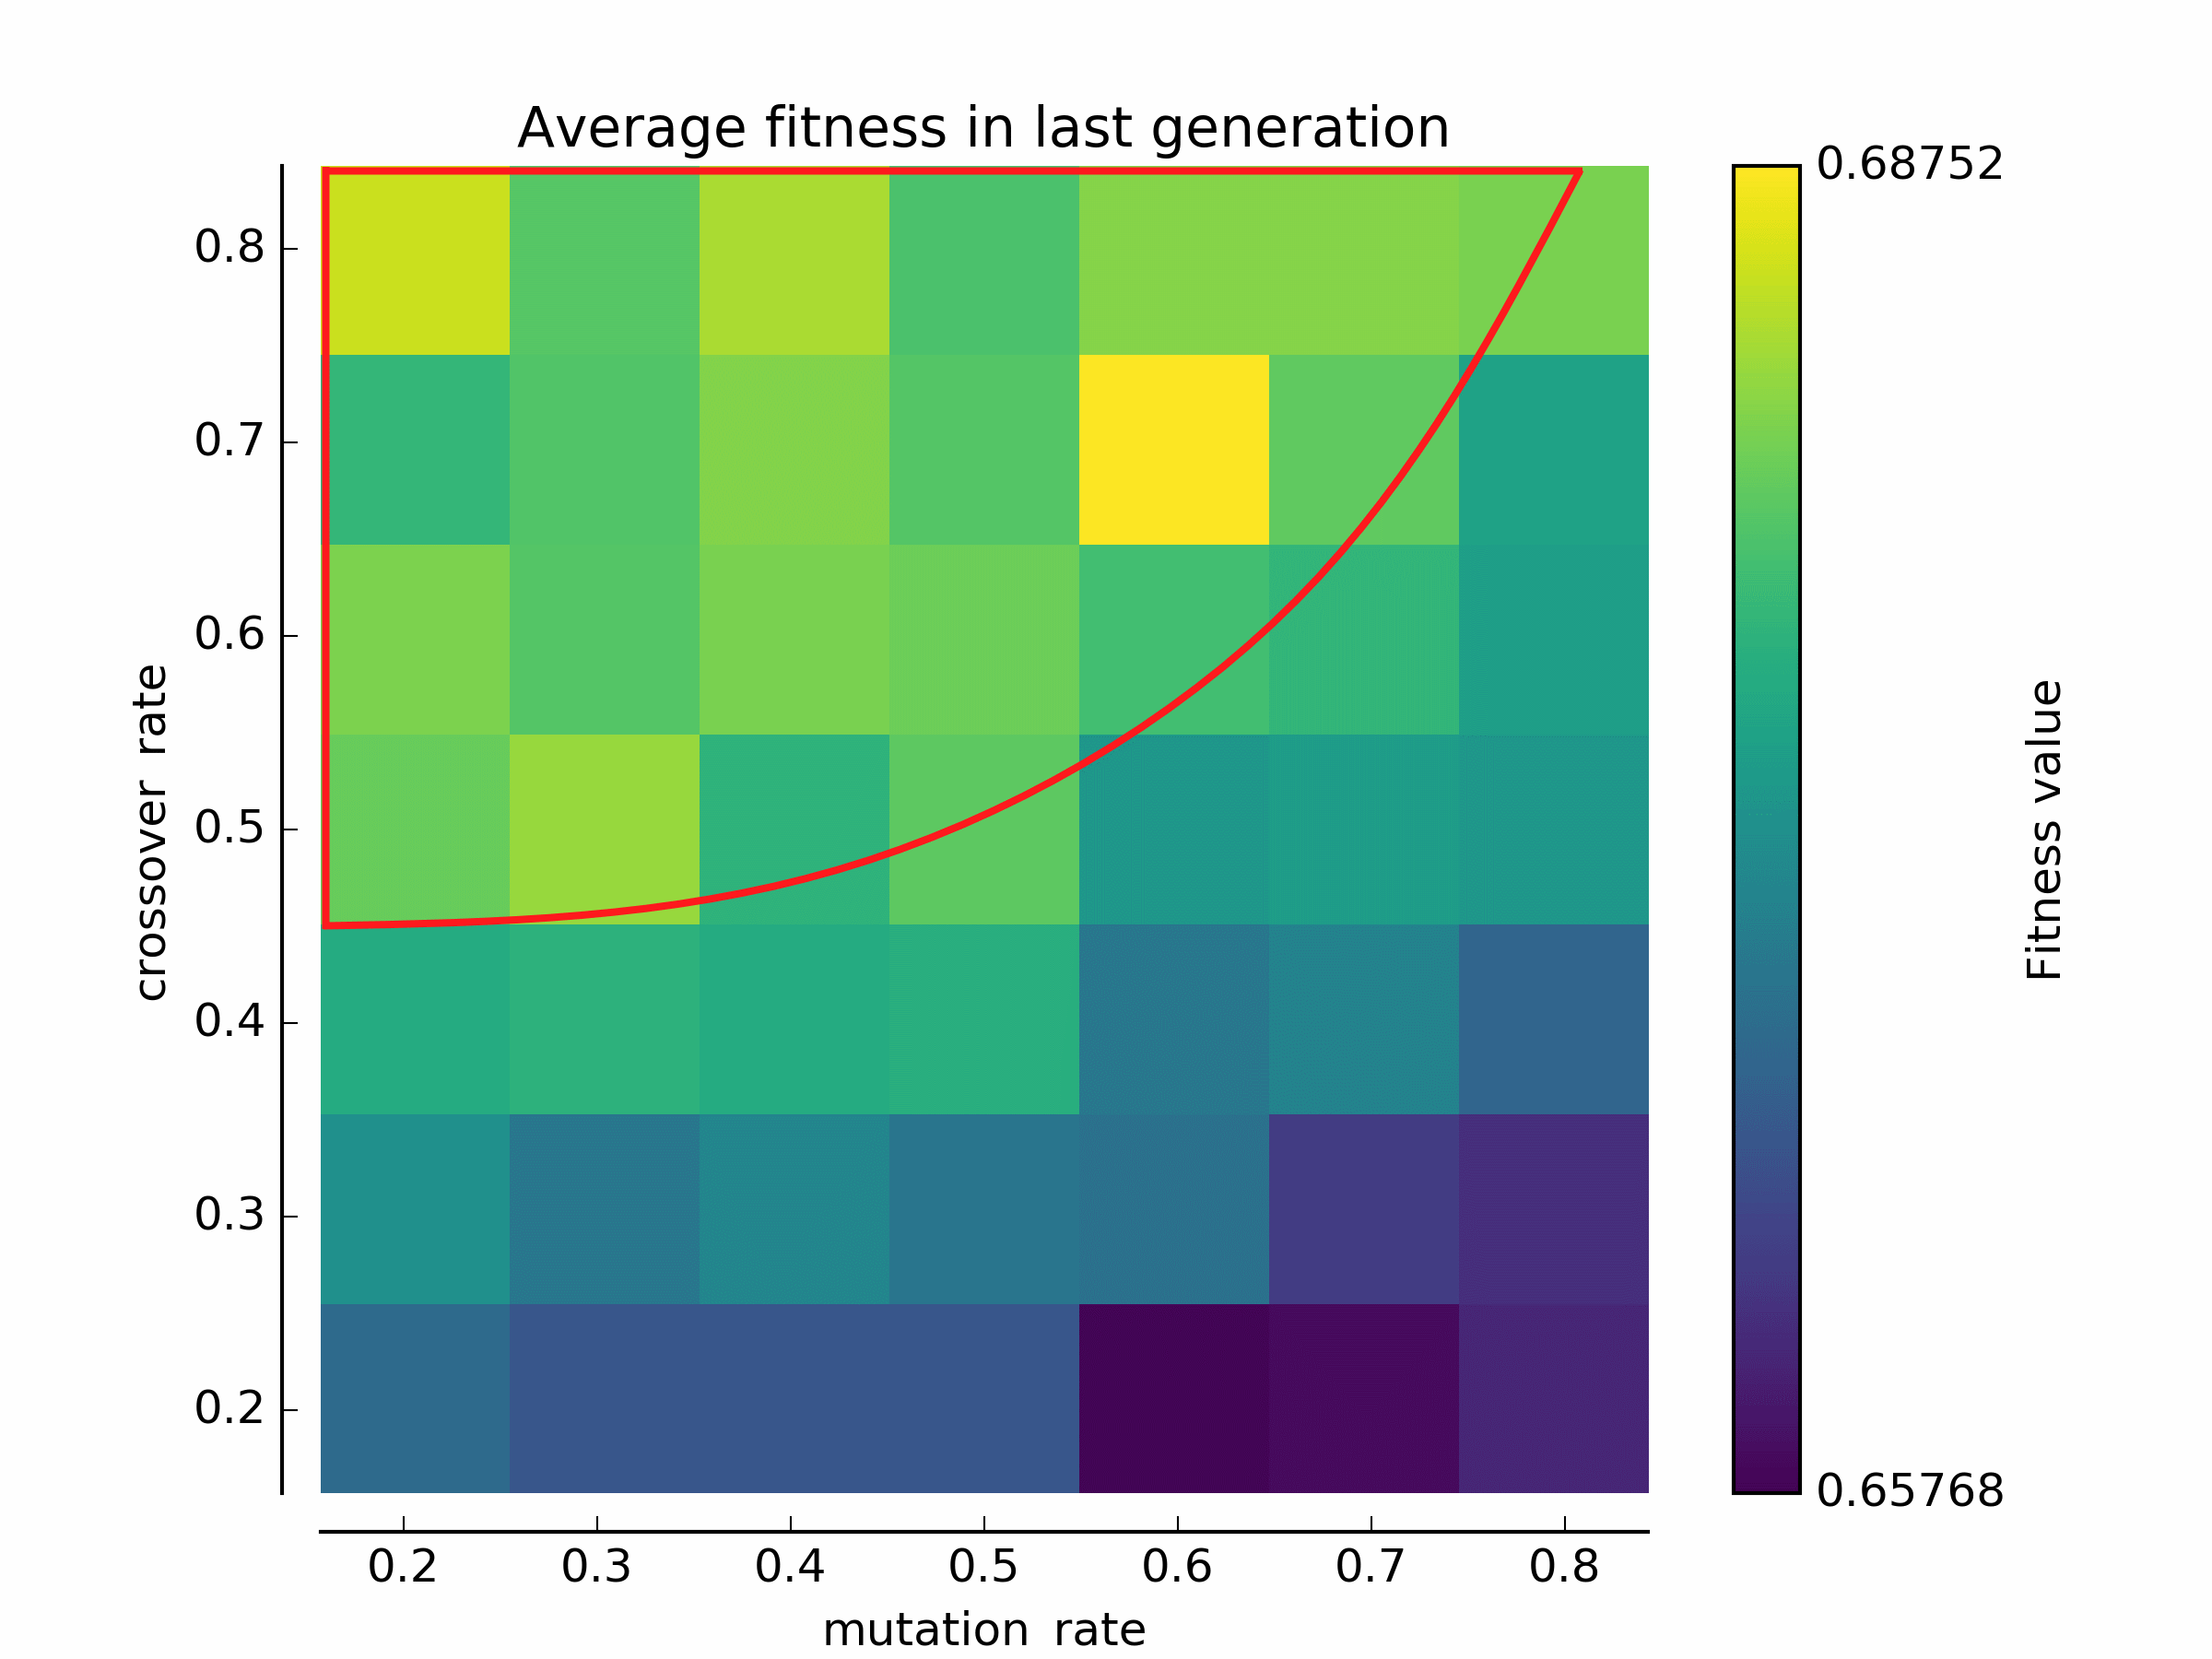
\includegraphics[width=0.99\textwidth]{grid_search_crossover_mutation_avg}
    \caption{The red region drawn on top of the heat map indicates the set of configurations deemed good}
    \label{fig:exp1_heatmap}
\end{figure}
% !TEX encoding = UTF-8 Unicode
%!TEX root = thesis.tex
% !TEX spellcheck = en-US
%%=========================================
\section{Experiment 2}
In this experiment, the aim is to find a good value for add link probability et al TODO

\subsection{Configuration}
\begin{minipage}{\linewidth}
\centering
\captionof{table}{Table Title TODO} \label{tab:title} 
\begin{tabular}{ C{3.5in} C{1.6in} }\toprule[1.5pt]
\bf Parameter & \bf Value \\
\midrule
  Number of generations & 50 \\
\midrule
  Fitness function & Local similarity \\
\midrule
  Target sound & Drum loop \\
\midrule
  Input sound & White noise \\
\midrule
  Effect & Distortion and resonant low-pass filter \\
\midrule
  Audio features & mfcc\_0, mfcc\_0\_\_derivative, mfcc\_1 \\
\midrule
  Number of runs & 400 per configuration \\
\bottomrule[1.25pt]
\end {tabular}\par
\bigskip
Should be a caption TODO
\end{minipage}

\subsection{Fitness function}
Same as in experiment 1

\subsection{Evaluation of configurations}
Figure \ref{fig:add_link_probability} TODO shows that 0.03 is probably the best value while 0.3 is significantly worse

\begin{figure}[h]
    \centering
    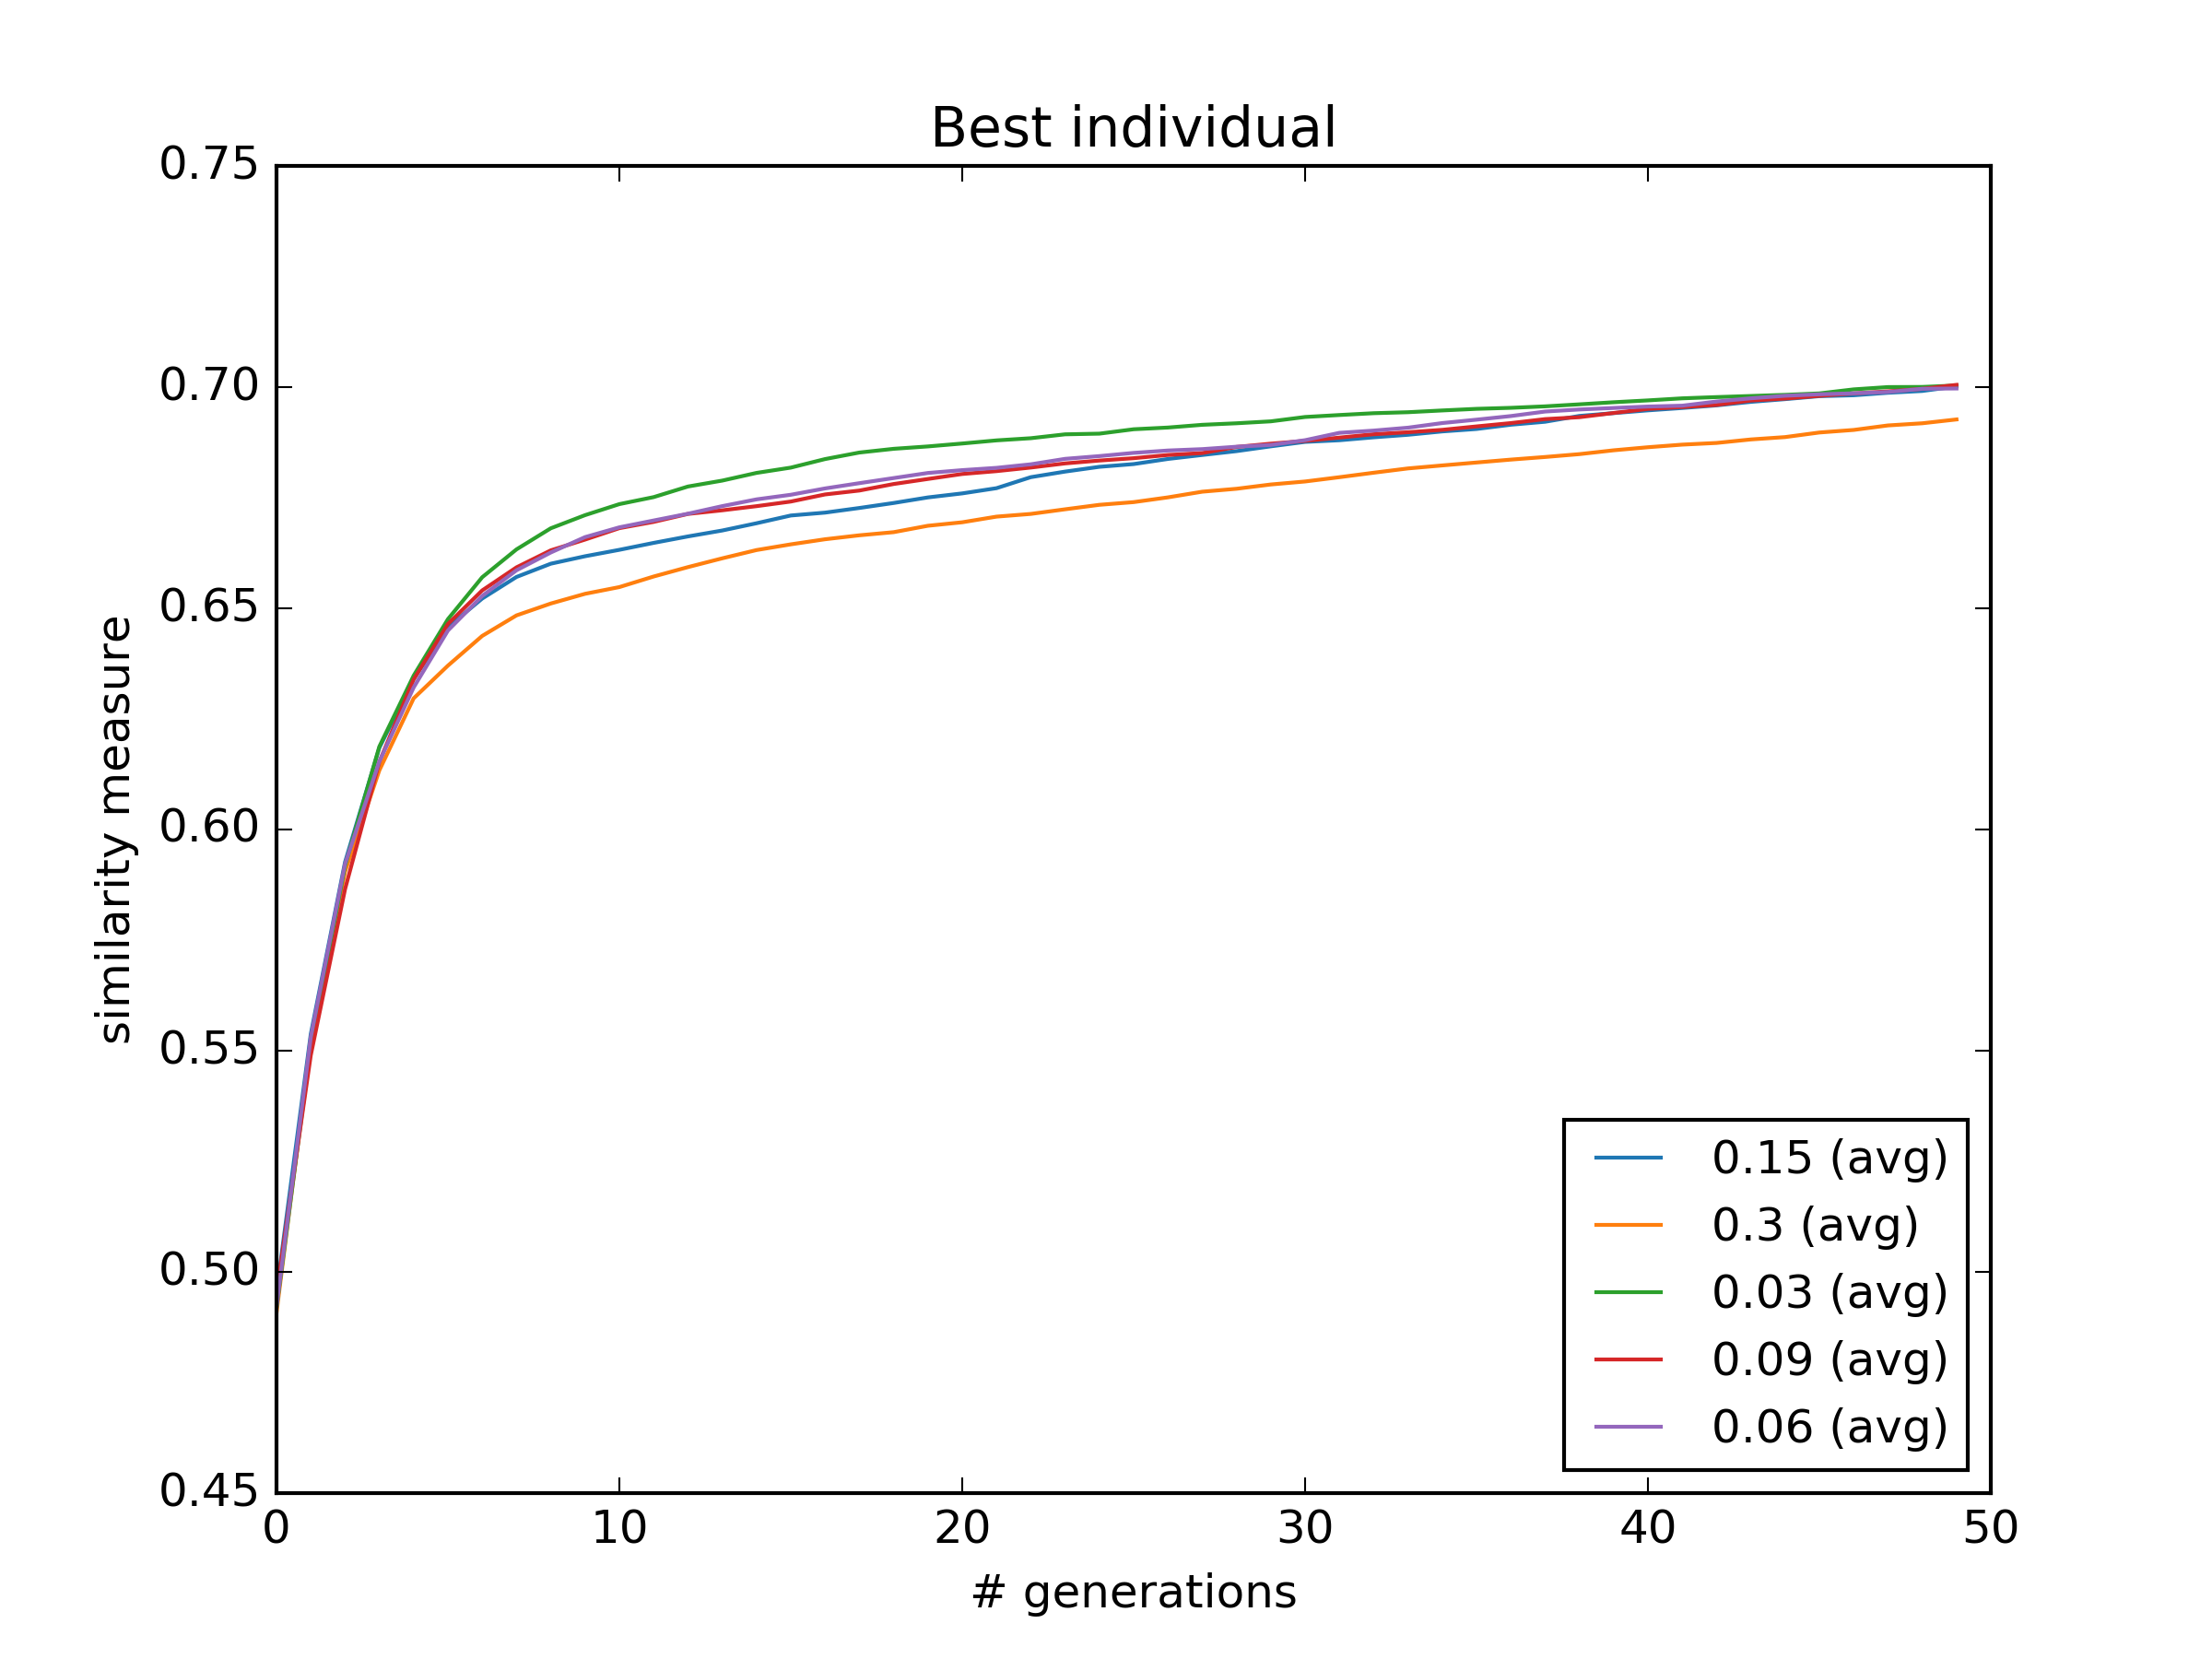
\includegraphics[width=0.99\textwidth]{add_link_probability}
    \caption{TODO caption}
    \label{fig:add_link_probability}
\end{figure}

TODO: Show typical end-result neural networks from all the configurations, to highlight that higher probability builds a larger, more complex network

% !TEX encoding = UTF-8 Unicode
%!TEX root = thesis.tex
% !TEX spellcheck = en-US
%%=========================================
\section{Experiment 3}
When using an evolved cross-adaptive audio effect in a live performance, a performer may want to use it in an expressive way. For example, if the performer is a drummer, he can vary the intensity of the drum hits. For the cross-adaptive audio effect to handle this, it needs to be trained on all the different intensities of the drum hits. If an extensive recording is available, that is fine. However, if the available target sound is short or lacks sufficient variation, one can harness the concept of data augmentation to create artificial variations of that sound. If one uses that sound instead, the evolved effect will typically be more capable of dealing with the generated variations. This experiment is about testing the author's implementation of data augmentation and the ability to apply evolved cross-adaptive audio effects to unseen sounds.

% TODO: mention the sounds and how augmented

\subsection{Configuration}

\begin{center}
\begin{longtable}{p{5cm} p{7cm}}
\caption[Experiment configuration]{Experiment configuration} \label{tab:exp3_configuration} \\

\hline \multicolumn{1}{l}{\textbf{Parameter}} & \multicolumn{1}{l}{\textbf{Value}} \\ \hline 
\endfirsthead

\multicolumn{2}{c}%
{{\bfseries \tablename\ \thetable{} -- continued from previous page}} \\
\hline \multicolumn{1}{l}{\textbf{Parameter}} & \multicolumn{1}{l}{\textbf{Value}} \\ \hline 
\endhead

\hline \multicolumn{2}{r}{{Continued on next page}} \\ \hline
\endfoot

\hline \hline
\endlastfoot

Number of generations & 20 \\
\midrule
Target sound (training) & Drum loop with bass drum, snare drum, clap and hihat (figure \ref{fig:exp3_waveforms}) \\
\midrule
Target sound (validation) & Snare roll (rapid snare drum hits) with ascending pitch and amplitude (figure \ref{fig:exp3_waveforms}) \\
\midrule
Input sound & White noise \\
\midrule
Effect & Distortion and resonant low-pass filter \\
\midrule
Audio features & Root Mean Square (RMS) and spectral centroid \\
\midrule
Number of runs & 40 per configuration \\
\end{longtable}
\end{center}

\begin{figure}[H]
    \centering
    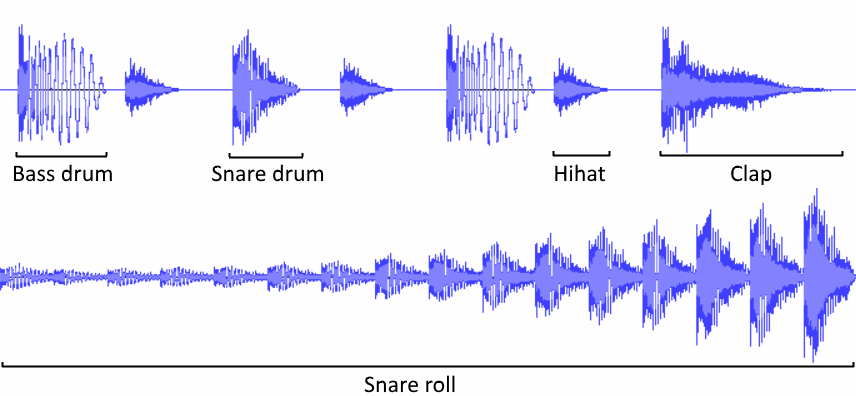
\includegraphics[width=1.0\textwidth]{exp3_waveforms}
    \caption{Waveform of training sound (top) and validation sound (bottom)}
    \label{fig:exp3_waveforms}
\end{figure}

The augmented variant of the training sound was created by repeating the sound 8 times, with variations in playback speed and gain for each repetition. The playback speed and gain are sampled from a gaussian distribution centered around $1$ and with standard deviations of $0.3$ and $0.5$, respectively.

%TODO: mention exponential thingy


\subsection{Results and evaluation}
Figure \ref{fig:exp3_fitness_box} shows that neural networks trained on an augmented variant of the training sound generalizes better than the raw training sound.

% Helps in live settings which typically play in more nuanced ways than the sounds the network is pre-trained on

\begin{figure}[H]
    \centering
    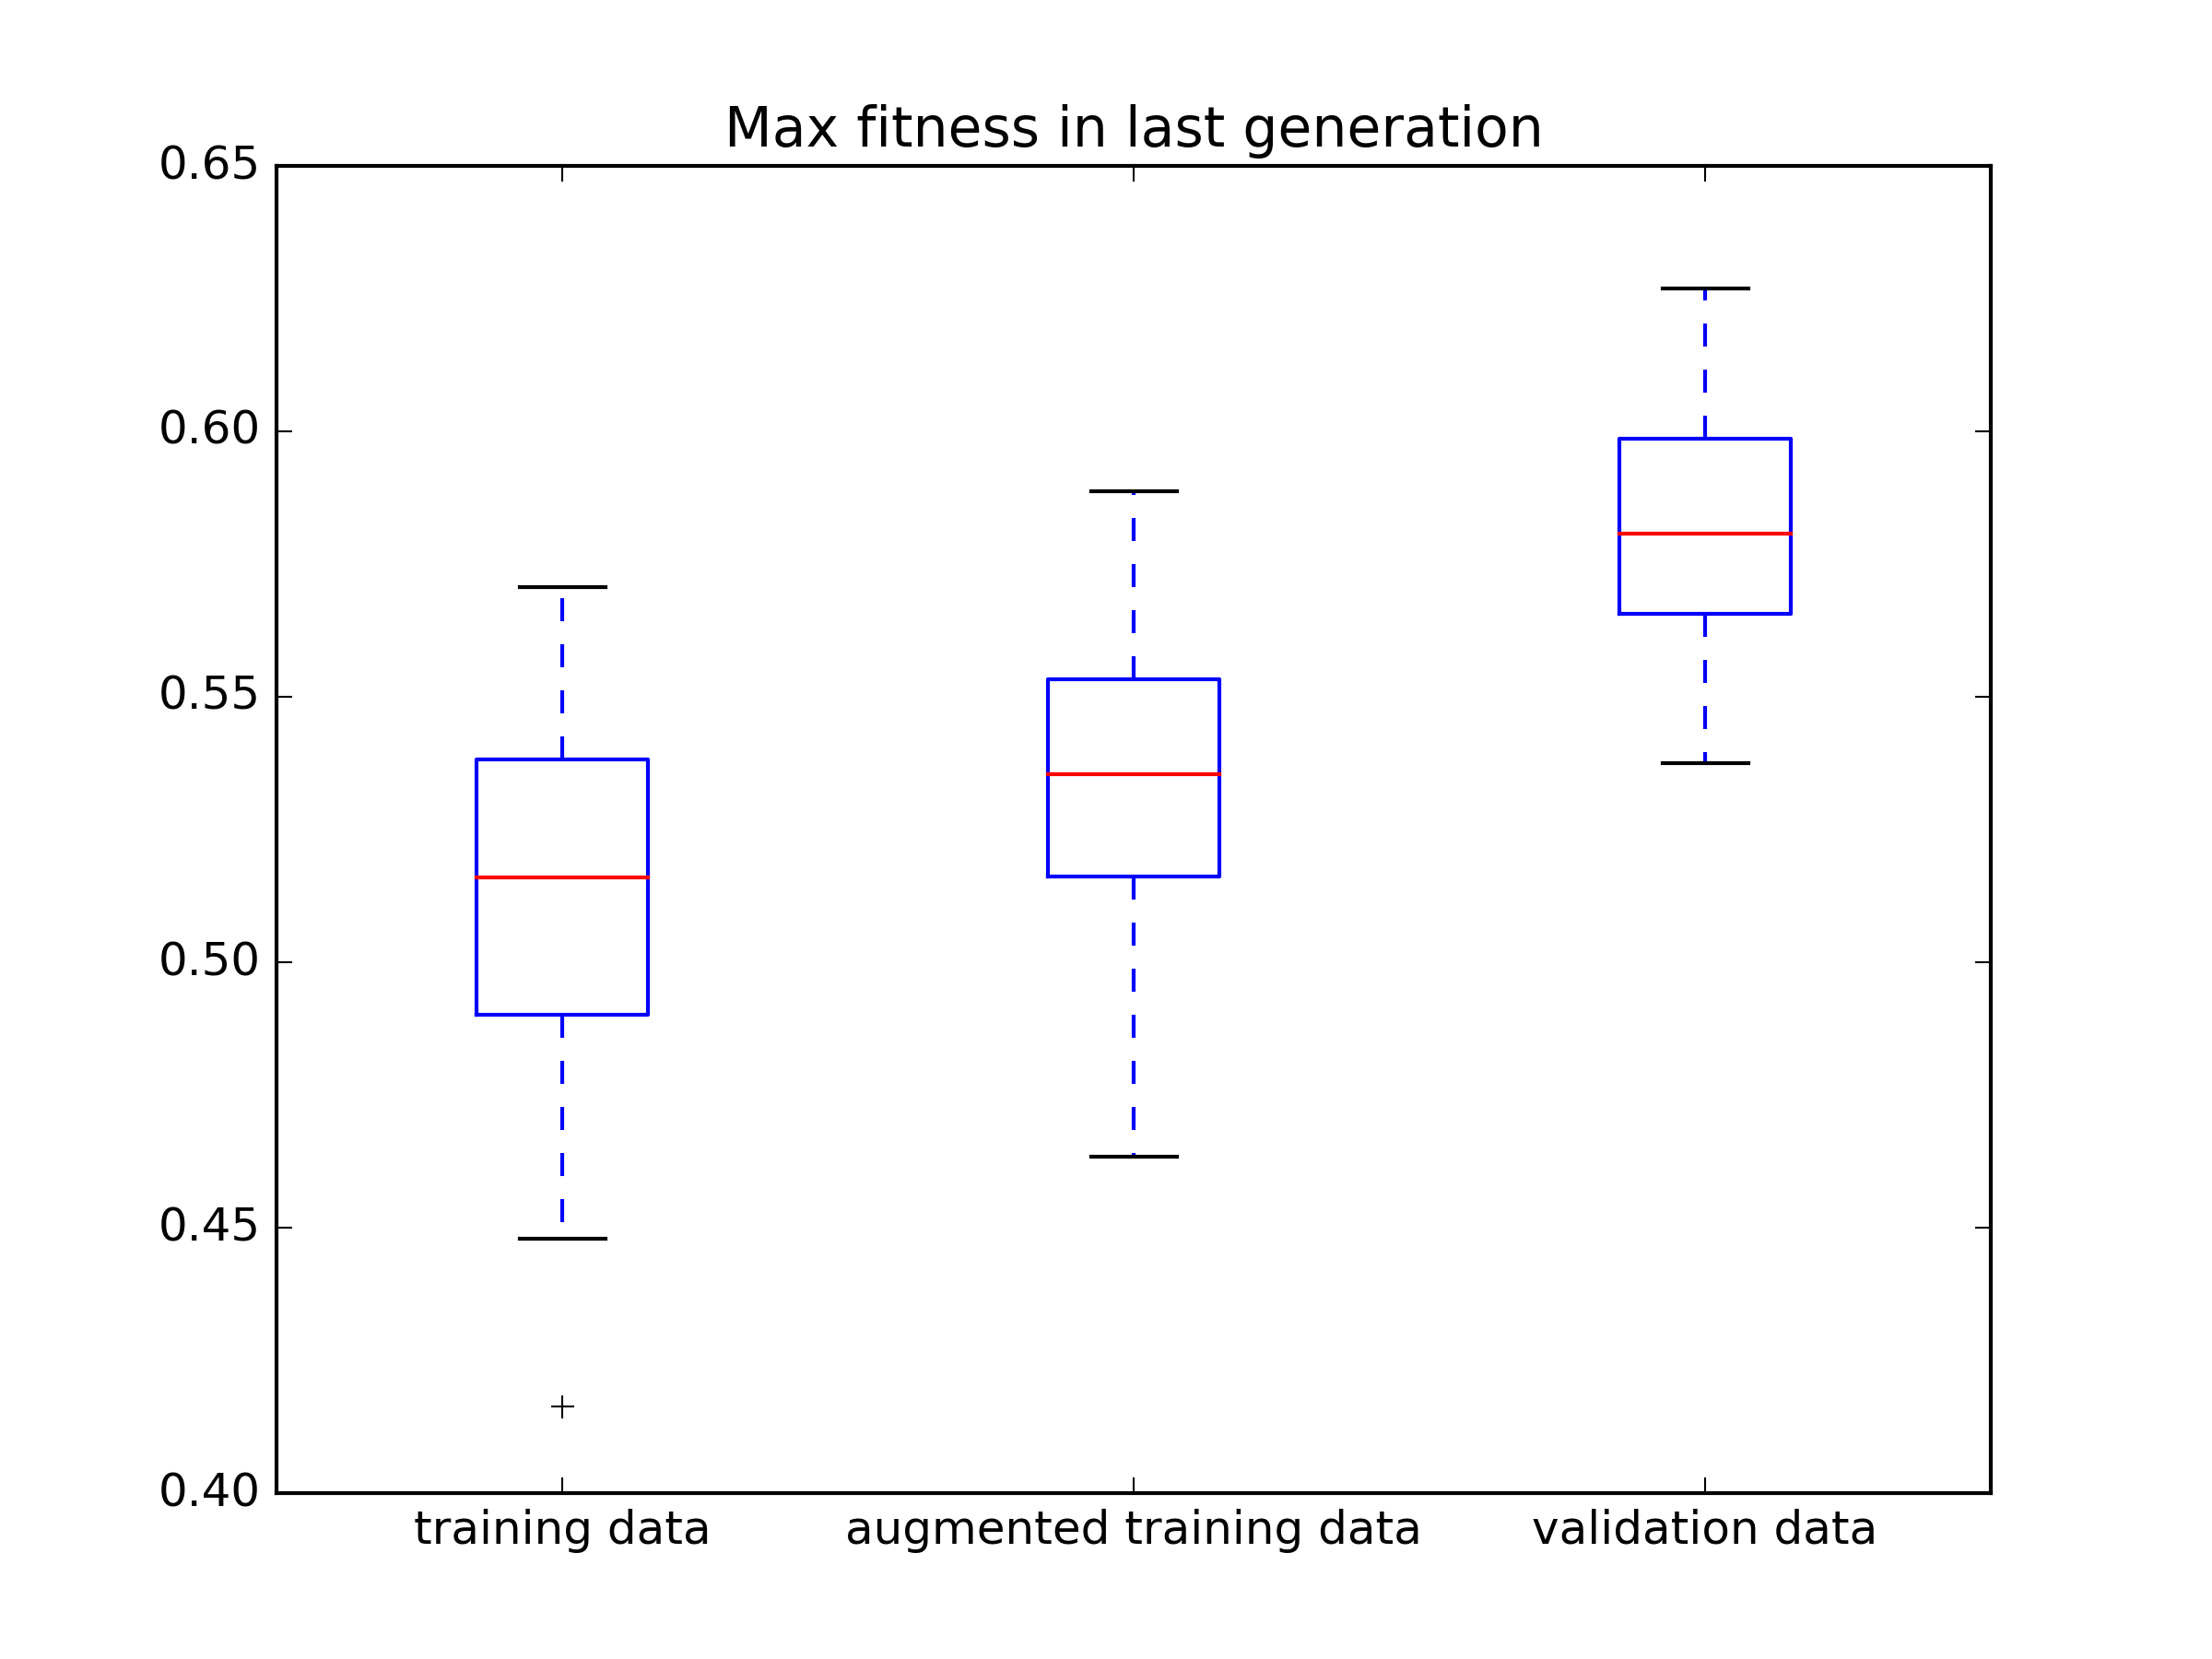
\includegraphics[width=1.0\textwidth]{exp3_fitness_box}
    \caption{Box plot of validation fitness values in final generation. The labels on the x-axis indicate which sound was used as target sound.}
    \label{fig:exp3_fitness_box}
\end{figure}

